\section{Cone}

\begin{frame}[fragile]{Definição}

    \begin{itemize}
        \item Um cone é uma figura geométrica formada pela união de todas as retas 
            (ou segmentos de retas) que unem uma base plana (uma região fechada) a um 
            ponto externo ao plano da base, denominado vértice ou \textit{apex}
        \pause

        \item O mais comum dentre os cones é o cone circular reto
        \pause

        \item No cone circular reto base é um círculo e o vértice está localizado na reta 
            perpendicular ao plano onde se encontra o círculo e que passa pelo centro do mesmo
        \pause

        \item Tal cone pode ser determinado pelo círculo da base (centro e raio) e pela distância 
            do vértice ao plano, denominada $H$
        \pause

        \item Se a localização exata do cone não for necessária, bastam apenas a distância $H$ e o 
            raio $r$ do círculo


    \end{itemize}

\end{frame}

\begin{frame}[fragile]{Visualização do cone circular reto}

    \begin{figure}
        \centering
        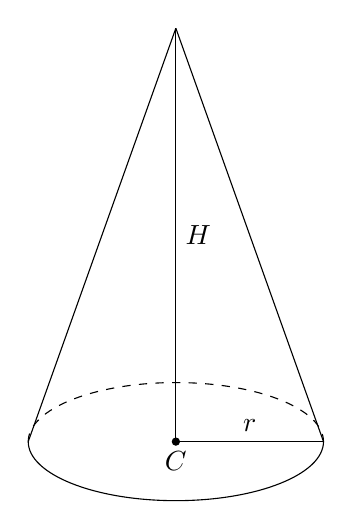
\begin{tikzpicture}[scale=1.5]
            \draw (0,0) -- (-1.25,-3.5);
            \draw (-1.25,-3.5) arc (180:360:1.25 and 0.5);
            \draw [dashed] (-1.25,-3.5) arc (180:360:1.25 and -0.5);
            \draw (1.25,-3.5) -- (0,0);  
            \draw (0,-3.5) -- node[anchor=west] { $H$ } (0,0);  
            \draw (0, -3.5) -- node[anchor=south] { $r$ } (1.25, -3.5);
            \fill (0, -3.5) circle [radius=1pt] node[anchor=north] { $C$ };
        \end{tikzpicture}
    \end{figure}

\end{frame}

\begin{frame}[fragile]{Área e volume}

    \begin{itemize}
        \item A área da superfície do cone circular reto é a soma da área da base mais 
            a área lateral, isto é,
        \[
            A = \pi r^2 + \pi r\sqrt{r^2 + H^2}
        \]
        \pause

        \item O valor $L = \sqrt{r^2 + H^2}$ surge do triângulo retângulo formado pelo vértice, 
            pelo centro e por um ponto do círculo
        \pause

        \item Se o cone for cortado num segmento de reta que une o círculo ao vértice e 
            aberto, ele resultará em um setor do círculo de raio $L$, cujo arco é $2\pi r$, 
            o que resulta em uma área lateral de $\pi rL$
        \pause

        \item O volume do cone circular reto pode ser computado através da integral de
            revolução em torno do eixo-$x$, com $0 \leq x \leq H$ e $f(x) = rx/H$, o que 
            resulta em 
            \[
                V = \int_0^H \pi f^2(x) dx = \frac{1}{3}\pi r^2 H
            \]

    \end{itemize}

\end{frame}

\begin{frame}[fragile]{Tronco do cone}

    \begin{itemize}
        \item O tronco de um cone é obtido através da seção de um cone por um plano paralelo à base
        \pause

        \item Se $R$ é o raio da base do cone, $r$ o raio do círculo resultante da seção e $h$ a 
            altura do tronco, o volume do tronco é dado por
        \[
            V = \frac{1}{3}\pi h(R^2 + Rr + r^2),
        \]
        \pause

        \item Este volume corresponde à diferença do volume do cone maior pelo volume do cone menor,
            obtido após à seção
        \pause

    \end{itemize}

    \begin{figure}
        \centering
        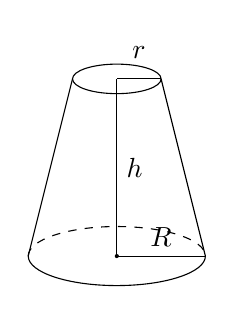
\begin{tikzpicture}[scale=0.75]
            \draw (0,0) ellipse (0.75 and 0.25);
            \draw (-0.75,0) -- (-1.5,-3.0);
            \draw (-1.5,-3.0) arc (180:360:1.5 and 0.5);
            \draw [dashed] (-1.5,-3.0) arc (180:360:1.5 and -0.5);
            \draw (1.5,-3.0) -- (0.75,0);  
            \draw (0.0,-3.0) -- node[anchor=west] { $h$ } (0.0,0);  
            \draw (0, -3.0) -- node[anchor=south] { $R$ } (1.5, -3.0);
            \draw (0, 0.0) -- node[anchor=south,inner sep=7pt] { $r$ } (0.75, 0.0);
            \fill (0, -3.0) circle [radius=1pt];
        \end{tikzpicture}
    \end{figure}

\end{frame}

\begin{frame}[fragile]{Implementação de um cone}
    \inputcode{cpp}{codes/cone.cpp}
\end{frame}
